%%%%%%%%%%%%%%%%%%%%%%%%%%%%%%%%%%%
%%%%%%%%%%%%%%%%%%%%%%%%%%%%%%%%%%%
\begin{frame}
  \frametitle{Main difference between CPU and GPU}
  
  \begin{center}
    \textbf{\textcolor{blue}{Architecture design differences between manycore GPUs and general purpose multicore CPU ?}}
    
    \only<1-4>{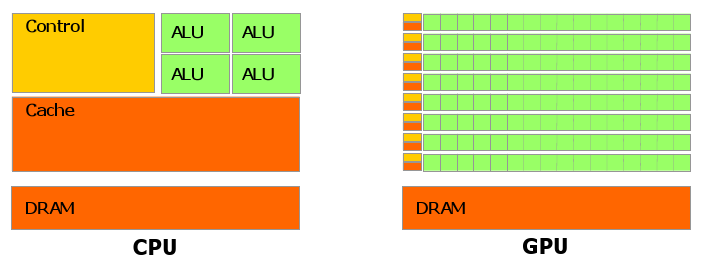
\includegraphics[height=3.5cm]{images/cpu_gpu_comparison}}

  \end{center}

\begin{itemize}

  \only<1>{
  \item \textbf{Different goals produce different designs:}
    \begin{itemize}
    \item \textcolor{red}{\textbf{CPU}}  must be good at everything, parallel or not
    \item \textcolor{blue}{\textbf{GPU}} assumes work load is highly parallel
    \end{itemize}
  }
  \only<2>{
  \item \textcolor{red}{\textbf{CPU}} design goal : optimize architecture for sequential code
    performance : \textcolor{red}{minimize latency experienced by \textbf{1 thread}}
    % latence = nb de cycle d'horloge pour acheminer des donnees de la memoire centrale jusqu'au coeur de calcul (ALU)
    % donner l'illusion d'une memoire tres rapide
    % exploiter la localite spatiale et temporelle de la memoire
    % s'il n'y avait pas de cache, les coeurs de proc serait sans arret en "stall"
    % voir l'article: http://dl.acm.org/citation.cfm?id=2692965.2682585
    % Rethinking caches for throughput processors: technical perspective
    % by Stephen W. Keckler
    
    \begin{itemize}
    \item \textcolor{red}{sophisticated} (i.e. large chip area) \textcolor{red}{control logic} for instruction-level parallelism
      (branch prediction, out-of-order instruction, etc...)
    \item \textcolor{red}{CPU have large cache memory} to reduce the instruction and
      data access latency
    \end{itemize}
  }

  \only<3>{
  \item \textcolor{blue}{\textbf{GPU}} design goal : \textcolor{blue}{maximize throughput of \textbf{all threads}}
    \begin{itemize}
    \item \# threads in flight limited by resources => lots of
      resources (registers, bandwidth, etc.)
    \item  multithreading can \textcolor{blue}{hide latency} => skip the big caches
    \item \textcolor{blue}{share control logic} across many threads
    \end{itemize}
  }

  \only<4>{
  \item \textcolor{red}{\bf CPU} : 1 thread $\Leftrightarrow$ 1 core
  \item \textcolor{blue}{\bf GPU}: nb threads $\gg$ nb cores
  }
\end{itemize}
  
\end{frame}

%%%%%%%%%%%%%%%%%%%%%%%%%%%%%%%%%%%%%%%%%%%%%%%% 
%%%%%%%%%%%%%%%%%%%%%%%%%%%%%%%%%%%%%%%%%%%%%%%% 
\begin{frame}
  \frametitle{Multidimensional array and data parallelism}

  \begin{center}
    \textcolor{violet}{\Large Memory layouts / index linearization: e.g. 2D}
  \end{center}
  
  \begin{columns}
    \begin{column}{0.5\textwidth}
      \begin{center}
        \textcolor{red}{\large row-major}
        
        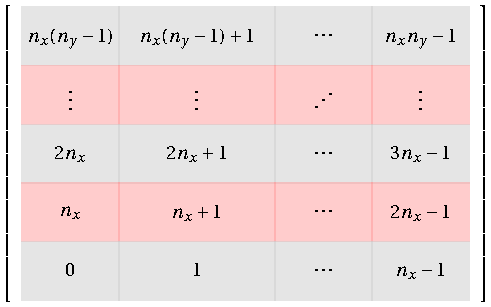
\includegraphics[width=5cm]{images/tikz/row-major}

        $\text{index} = i + n_x j$, \textcolor{red}{left layout}\\
        fast index on the left
      \end{center}
    \end{column}
    % 
    \begin{column}{0.5\textwidth}
      \begin{center}
        \textcolor{blue}{\large column-major}
        
        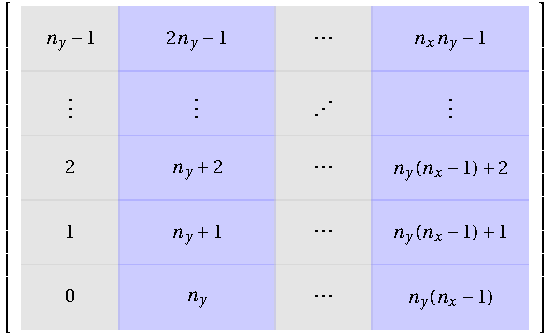
\includegraphics[width=5cm]{images/tikz/col-major}        

        $\text{index} = j + n_y i$, \textcolor{blue}{right layout}\\
        fast index on the right
      \end{center}
    \end{column}
  \end{columns}

\end{frame}

%%%%%%%%%%%%%%%%%%%%%%%%%%%%%%%%%%%%%%%%%%%%%%%% 
%%%%%%%%%%%%%%%%%%%%%%%%%%%%%%%%%%%%%%%%%%%%%%%% 
\begin{frame}[fragile=singleslide]
  \frametitle{Multidimensional array and data parallelism}

  \begin{block}{}
    {\large \textcolor{violet}{Question:}
    Assuming \textcolor{red}{left layout}, which loop would you prefer to parallelize (inner or outer) ?}    
  \end{block}
  
  \begin{columns}
    \begin{column}{0.45\textwidth}
      \begin{center}
        \textcolor{red}{\large row-major}
        
        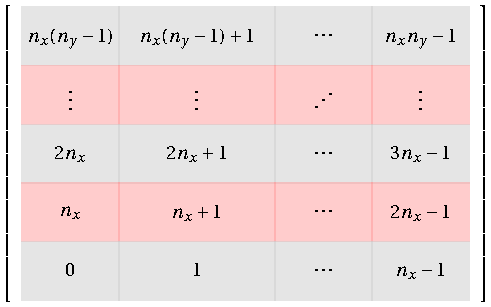
\includegraphics[width=5cm]{images/tikz/row-major}

        $\text{index} = i + n_x j$, \textcolor{red}{left layout}\\
        fast index on the left
      \end{center}
    \end{column}
    %\hspace{-1.5cm}
    \begin{column}{0.48\textwidth}
\begin{minted}{c++}
  for(int j=0; j<ny; ++j)
    for(int i=0; i<nx; ++i)
      data[i+nx*j] += 12;
\end{minted}
\begin{center}
  \textcolor{blue}{\bf Favor memory locality:}
\end{center}
\begin{itemize}
\item maximize cache usage for CPU
\item maximize memory coalescence on GPU
\end{itemize}
\begin{center}
  \textcolor{darkgreen}{\bf Different hardware $\Rightarrow$ \\ different parallelization strategies}
\end{center}
\end{column}
    \hfill
  \end{columns}
\end{frame}

%%%%%%%%%%%%%%%%%%%%%%%%%%%%%%%%%%%%%%%%%%%%%%%% 
%%%%%%%%%%%%%%%%%%%%%%%%%%%%%%%%%%%%%%%%%%%%%%%% 
\begin{frame}[fragile=singleslide]
  \frametitle{Multidimensional array and data parallelism}

  \begin{block}{}
    {\large \textcolor{violet}{Question:}
    Assuming \textcolor{red}{left layout}, which loop would you prefer to parallelize (inner or outer) ?}    
  \end{block}
  
  \begin{columns}
    \begin{column}{0.48\textwidth}
      \begin{center}
        \textcolor{red}{\large row-major}
        
        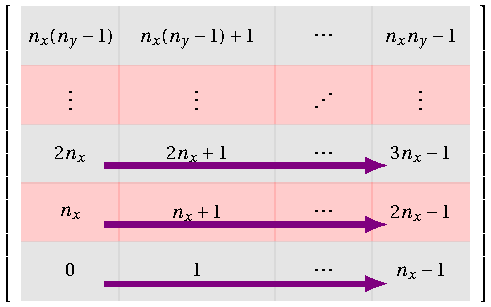
\includegraphics[width=5cm]{images/tikz/row-major-openmp}

        $\text{index} = i + n_x j$, \textcolor{red}{left layout}\\
        fast index on the left
      \end{center}
    \end{column}
    %\hspace{-1.0cm}
    \begin{column}{0.48\textwidth}
      \begin{center}
        \textcolor{violet}{\bf OpenMP // outer loop}\\
        each OpenMP thread handles {\bf 1 or more row(s)}
      \end{center}
      \begin{minted}{c++}
#pragma omp parallel
{
  #pragma omp for
  for(int j=0; j<ny; ++j)

    // vectorization loop
    // memory contiguity
    for(int i=0; i<nx; ++i)
      data[i+nx*j] += 12;
}
      \end{minted}
    \end{column}
    \hfill
  \end{columns}
\end{frame}

%%%%%%%%%%%%%%%%%%%%%%%%%%%%%%%%%%%%%%%%%%%%%%%% 
%%%%%%%%%%%%%%%%%%%%%%%%%%%%%%%%%%%%%%%%%%%%%%%% 
\begin{frame}[fragile=singleslide]
  \frametitle{Multidimensional array and data parallelism}

  \begin{block}{}
    {\large \textcolor{violet}{Question:}
    Assuming \textcolor{red}{left layout}, which loop would you prefer to parallelize (inner or outer) ?}    
  \end{block}
  
  \begin{columns}
    \begin{column}{0.48\textwidth}
      \begin{center}
        \textcolor{red}{\large row-major}
        
        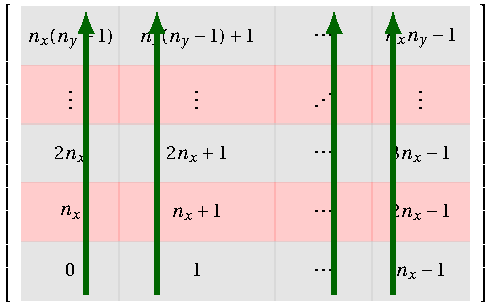
\includegraphics[width=5cm]{images/tikz/row-major-cuda}

        $\text{index} = i + n_x j$, \textcolor{red}{left layout}\\
        fast index on the left
      \end{center}
    \end{column}
    %\hspace{-1.0cm}
    \begin{column}{0.48\textwidth}
      \begin{center}
        \textcolor{darkgreen}{\bf CUDA // inner loop}\\
        each CUDA thread handles {\bf1 or more col(s)}\\
        memory coalescence
      \end{center}
      {\small
        \begin{minted}[autogobble=true]{c++}
__global__ void compute(int *data)
{
  // adjacent memory cells
  // computed by
  // neighboring threads
  int i = threadIdx.x +
      blockIdx.x*blockDim.x;
  
  for(int j=0; j<ny; ++j)
    data[i+nx*j] += 12;
}
\end{minted}
}
    \end{column}
    \hfill
  \end{columns}
\end{frame}

%%%%%%%%%%%%%%%%%%%%%%%%%%%%%%%%%%%%%%%%%%%%%%%% 
%%%%%%%%%%%%%%%%%%%%%%%%%%%%%%%%%%%%%%%%%%%%%%%% 
\begin{frame}[fragile=singleslide]
  \frametitle{Multidimensional array and data parallelism}

  \begin{block}{Conclusion}
    {\Large Don't assume \textcolor{red}{layout}, let's \textcolor{red}{chose} at compile-time !}
  \end{block}
  
  \begin{itemize}
  \item {\bf First conclusion:}\\
    if we keep the same memory layout, \textcolor{violet}{\bf OpenMP} and \textcolor{darkgreen}{\bf CUDA} \textcolor{red}{\bf disagree} on which loop should be parallelized to optimize for their respective hardware target.
  \item \textcolor{blue}{\bf How can we make portable code ?}
  \item Note that swapping memory layout and {\tt for loops} is {\bf involutive}
  %\item instead of swapping loops, swap memory layout
  \item \textcolor{orange}{\bf Kokkos answer:} make memory layout abstract (since a good memory layout is hardware dependent), fixed at compile-time\\
    access $data(i,j)$
    \begin{itemize}
    \item On \textcolor{violet}{\bf OpenMP} $data(i,j)$ actually means accessing $dataPtr[Ny*i+j]$
    \item On \textcolor{darkgreen}{\bf Cuda} $data(i,j)$ actually means accessing $dataPtr[i+Nx*j]$
    \end{itemize}
  \end{itemize}
  
\end{frame}

%%%%%%%%%%%%%%%%%%%%%%%%%%%%%%%%%%%%%%%%%%%%%%%% 
%%%%%%%%%%%%%%%%%%%%%%%%%%%%%%%%%%%%%%%%%%%%%%%% 
\begin{frame}[fragile=singleslide]
  \frametitle{Multidimensional array and data parallelism}

  \begin{block}{Conclusion}
    {\Large Don't assume \textcolor{red}{layout}, let's \textcolor{red}{chose} at compile-time !\\
    $\Rightarrow$ \textcolor{red}{\textbf{and make it hardware aware.}}}
  \end{block}
  
  \begin{columns}
    \begin{column}{0.45\textwidth}
      \begin{center}
        \textcolor{black}{\large left layout / CUDA}\\
        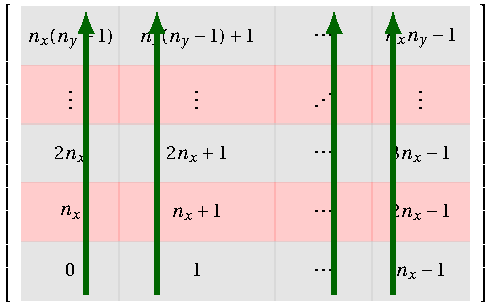
\includegraphics[width=2.8cm]{images/tikz/row-major-cuda}

        \textcolor{black}{\large right layout / OpenMP}\\
        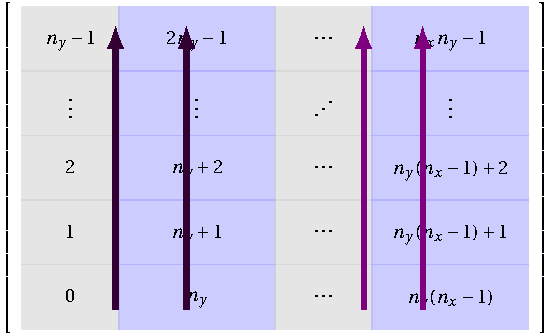
\includegraphics[width=2.8cm]{images/tikz/col-major-kokkos-openmp}

      \end{center}
    \end{column}
    %\hspace{-1.5cm}
    \begin{column}{0.45\textwidth}
      \begin{center}
        \textcolor{orange}{\bf Kokkos parallel version for both CUDA/OpenMP}
      \end{center}
      \begin{minted}{c++}
Kokkos::parallel_for(nx,
   KOKKOS_LAMBDA(int i) {
     for (int j=0; j<ny; ++j)
       data(i,j) += 12;
   }
);
      \end{minted}
    \end{column}
    \hfill
  \end{columns}
\end{frame}
